\chapter{Architektura systému}

\section{Architektonický vzor}

Mobilní aplikace LifeMeter je vytvořena v prostředí React Native s využitím platformy Expo. Namísto nativního vývoje pro Android byl zvolen tento technologický stack zejména z důvodu potenciální budoucí kompatibility s~platformou iOS, přičemž přechod na nativní aplikaci by vyžadoval zásadní přepsání kódové základny. Dalším faktorem bylo, že vývoj v~jazyce TypeScript a~frameworku React umožnil výrazně efektivnější implementaci oproti nativnímu Androidu s~využitím jazyka Kotlin, s~nímž nebyly k~dispozici dostatečné předchozí zkušenosti.

Architektura aplikace vychází z návrhového vzoru \textbf{MVC} (Model--View--Controller)~\cite{torres2021mvc}, který je přizpůsoben prostředí React Native. Jednotlivé vrstvy odpovídají následujícímu rozdělení zodpovědností:
\begin{itemize}
    \item \textbf{Model:} Servisní třídy (\texttt{sleep.service.ts}, \texttt{food.service.ts}, ...) zapouzdřují veškerou komunikaci se vzdáleným API serverem. Každá třída odpovídá jedné doménové oblasti a~poskytuje typované metody pro CRUD operace nad příslušnými zdroji.
    \item \textbf{View:} Obrazovky a~komponenty implementované v~souborech \texttt{.tsx} tvoří prezentační vrstvu. Komponenty jsou čistě zobrazovací; žádná business logika ani přímá komunikace se serverem v~nich není přítomna.
    \item \textbf{Controller:} Globální stavové kontexty \texttt{useStore} a~\texttt{useAuth} plní roli controlleru. Kontext \texttt{useAuth} řídí stav autentizace a~životní cyklus relace, zatímco \texttt{useStore} agreguje data všech domén (spánek, jídlo, tréninky, profil) a~vystavuje akce, které komponenty volají prostřednictvím hooků React.
\end{itemize}

\begin{figure}[H]
    \centering
    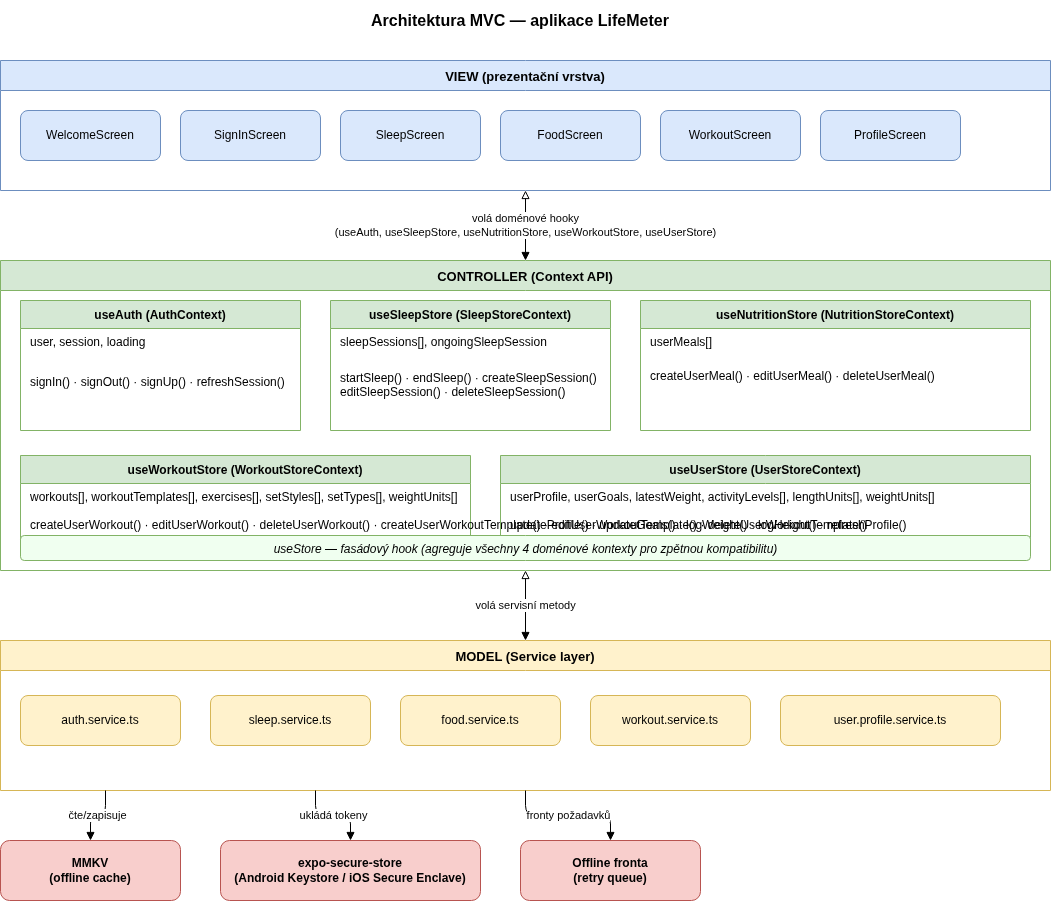
\includegraphics[width=0.82\textwidth]{references/img/architecture/mvc_schema.png}
    \caption{Schéma architektonického vzoru MVC aplikace LifeMeter}
    \label{fig:mvc_schema}
\end{figure}

% -------------------------------------------------------------------
\subsection{Popis vrstev aplikace}
% -------------------------------------------------------------------

\subsubsection*{Prezentační vrstva (View)}

Prezentační vrstva se skládá z~obrazovek organizovaných do adresářů
podle funkčních oblastí (\texttt{sleep}, \texttt{food}, \texttt{workout},
\texttt{onboarding}, \texttt{profile}). Navigace mezi obrazovkami
je zajištěna knihovnou \texttt{@react-navigation} prostřednictvím
nativního zásobníku obrazovek (\texttt{createNativeStackNavigator})
a~spodní lišty karet (\texttt{createBottomTabNavigator}).
Komponenty jsou stylizovány pomocí knihovny Tailwind CSS adaptované
pro React Native prostřednictvím balíčku \texttt{uniwind} a~komponentové
knihovny \texttt{heroui-native}.

\subsubsection*{Vrstva controlleru (Context)}

Stav aplikace je spravován pomocí React Context API, přičemž globální
stav je rozdělen do pěti samostatných kontextů. Toto rozdělení zamezuje
zbytečnému překreslování komponent při změně stavu v~jedné doméně.

\begin{itemize}
    \item \texttt{AuthContext} (\texttt{useAuth}): uchovává referenci na přihlášeného uživatele a aktivní relaci, zprostředkovává operace přihlášení, odhlášení a registrace a reaguje na výsledek volání \texttt{auth.service.ts}.
    \item \texttt{SleepStoreContext} (\texttt{useSleepStore}): spravuje záznamy spánku; vystavuje akce \texttt{startSleep}, \texttt{endSleep}, \texttt{createSleepSession}, \texttt{editSleepSession} a \texttt{deleteSleepSession}.
    \item \texttt{NutritionStoreContext} (\texttt{useNutritionStore}): spravuje záznamy jídla (user meals); vystavuje akce \texttt{createUserMeal}, \texttt{editUserMeal} a \texttt{deleteUserMeal}.
    \item \texttt{WorkoutStoreContext} (\texttt{useWorkoutStore}): spravuje záznamy tréninků a šablony tréninků; vystavuje akce  \texttt{createUserWorkout}, \texttt{editUserWorkout}, \texttt{deleteUserWorkout}, \texttt{createUserWorkoutTemplate} a obdobné operace nad šablonami.
    \item \texttt{UserStoreContext} (\texttt{useUserStore}): spravuje profil uživatele, cíle, váhové záznamy a referenční číselníky (jednotky hmotnosti a délky, úrovně aktivity); vystavuje akce \texttt{updateProfile}, \texttt{updateGoals}, \texttt{logWeight} a \texttt{logHeight}.
\end{itemize}

Pro zpětnou kompatibilitu existuje také fasádový hook \texttt{useStore},
který agreguje výstupy všech čtyř doménových kontextů do jediného
rozhraní. Jeho použití však způsobuje překreslení komponenty při změně
v~jakékoli doméně, proto je ve výkonnostně kritických obrazovkách
doporučeno volat doménové hooky přímo.

\subsubsection*{Datová vrstva (Model / Services)}

Datová vrstva tvoří rozhraní mezi aplikací a vzdáleným REST API
serverem na adrese \texttt{https://lifemeter.fit}. Komunikace probíhá
prostřednictvím pěti servisních tříd — \texttt{auth.service.ts},
\texttt{sleep.service.ts}, \texttt{food.service.ts},
\texttt{workout.service.ts} a~\texttt{user.profile.service.ts} —
z~nichž každá zapouzdřuje veškeré volání API pro příslušnou doménu.
Všechny servisní třídy sdílejí pomocné funkce \texttt{request()}
a~\texttt{fetchWithTimeout()}, jež obalují nativní \texttt{fetch}
API a~zajišťují jednotné zpracování chyb a~časových limitů.

Autentizace je řešena prostřednictvím knihovny Better Auth
s~relacemi na bázi cookies (\texttt{credentials: 'include'}).
Citlivé uživatelské údaje (například přihlašovací token) jsou
ukládány do zabezpečeného úložiště platformy pomocí
\texttt{expo-secure-store}, které na Androidu využívá
Android Keystore, respektive iOS Secure Enclave na platformě iOS.

\subsubsection*{Offline vrstva a fronta požadavků~\cite{androiddev2026offline}}

Aplikace podporuje offline režim prostřednictvím lokálního úložiště
\textbf{MMKV}, jež poskytuje vysokorychlostní synchronní přístup
k~perzistentním datům přímo z~vlákna JavaScriptu bez blokování
hlavního vlákna UI. Při startu aplikace jsou data načítána ze serveru;
v~případě nedostupnosti sítě jsou zobrazena lokálně uložená data.

Operace, jejichž provedení selhalo z~důvodu nedostupnosti připojení,
jsou zařazeny do \textbf{offline fronty}. Po obnovení konektivity
jsou požadavky z~fronty automaticky opětovně odeslány, čímž je
zajištěna konzistence dat mezi lokálním stavem aplikace a~serverem.

\subsubsection*{Backend}

Serverová část aplikace je tvořena REST API postaveným na frameworku
\textbf{Hono} s~runtime prostředím \textbf{Bun}. Databáze je
provozována na PostgreSQL 17. Server je trvale nasazen na adrese
\texttt{https://lifemeter.fit} prostřednictvím Docker Compose
na virtuálním stroji Oracle Cloud. Nasazení nové verze je
automatizováno prostřednictvím GitHub Actions, které při každém
pushnutí do větve \texttt{main} provede aktualizaci serveru
přes SSH. Přehled komunikace mezi klientem a~serverem je
znázorněn na obrázku~\ref{fig:system_overview}.

\begin{figure}[H]
    \centering
    
\includegraphics[width=0.85\textwidth]{references/img/architecture/system_overview.png}
    \caption{Komunikace mezi klientem a serverem aplikace LifeMeter}
    \label{fig:system_overview}
\end{figure}

% -----------------------------------------------------------------------
\section{Přehled komponent systému}
% -----------------------------------------------------------------------

Systém LifeMeter se skládá ze čtyř hlavních skupin komponent: mobilního
klienta, serverové části, externích zdravotních platforem a~lokálních
úložišť na straně zařízení. Jejich vzájemné vztahy jsou znázorněny
na obrázku~\ref{fig:components}.

\begin{figure}[H]
    \centering
    % \includegraphics[width=0.85\textwidth]{references/img/architecture/components.png}
    \caption{Přehled komponent systému LifeMeter}
    \label{fig:components}
\end{figure}

\subsection*{Mobilní klient}

Mobilní klient je implementován v~prostředí React Native s~platformou
Expo a~tvoří jedinou vstupní bránu, skrze níž uživatel interaguje
s~celým systémem. Klient zajišťuje prezentaci dat, správu
globálního stavu prostřednictvím kontextu \texttt{AuthContext}
a~čtyř doménových kontextů (\texttt{SleepStoreContext},
\texttt{NutritionStoreContext}, \texttt{WorkoutStoreContext},
\texttt{UserStoreContext}), navigaci mezi obrazovkami a~koordinaci
všech ostatních komponent popsaných níže.

\subsection*{REST API server}

Serverová část je postavena na frameworku \textbf{Hono} s~runtime
prostředím \textbf{Bun} a~je dostupná na adrese
\texttt{https://lifemeter.fit}. Server plní roli centrálního bodu
zpracování business logiky: přijímá požadavky od mobilního klienta,
ověřuje autentizaci, provádí validaci vstupních dat a~zprostředkovává
přístup k~databázi. Veškerá komunikace mezi klientem a~serverem
probíhá prostřednictvím protokolu HTTPS.

\subsection*{PostgreSQL 17}

Primárním datovým úložištěm na straně serveru je relační databáze
\textbf{PostgreSQL 17}. Jsou v~ní uloženy veškeré uživatelské záznamy
(spánek, jídlo, tréninky, profil, cíle, váhové záznamy), referenční
číselník potravin a~data správy relací spravovaná knihovnou Better Auth.
Přístup k~databázi probíhá výhradně přes API server; klient k~ní
nemá přímý přístup.

\subsection*{MMKV — lokální úložiště}

Na straně klienta slouží knihovna \textbf{MMKV} jako vysokorychlostní
perzistentní cache serverových dat. Data jsou do MMKV zapsána po každém
úspěšném načtení ze serveru a~při nedostupnosti sítě jsou z~ní čtena,
čímž je zajištěn offline přístup k~posledním známým datům. MMKV rovněž
uchovává serializovanou frontu neodoslaných mutačních požadavků
(viz sekci~\ref{sec:offline}).

\subsection*{expo-secure-store}

Citlivé přihlašovací údaje, zejména session token vydaný serverem,
jsou ukládány prostřednictvím knihovny \textbf{expo-secure-store}.
Ta na platformě Android využívá systémové úložiště Android Keystore,
na platformě iOS pak Secure Enclave. Díky tomu nejsou citlivé údaje
nikdy ukládány do nezabezpečených úložišť, jako jsou MMKV nebo
AsyncStorage.

\subsection*{Health Connect a Apple HealthKit}

Za účelem rozšíření zdrojů zdravotních dat jsou integrovány dvě
platformní zdravotní služby. Na platformě Android je využíváno
\textbf{Health Connect}, standardizované rozhraní systému Android
pro výměnu zdravotních dat mezi aplikacemi. Na platformě iOS
plní ekvivalentní roli \textbf{Apple HealthKit}. Obě integrace
umožňují číst data naměřená třetími stranami (například krokoměry,
spánkové trackery nebo sportovní hodinky) a~importovat je do
aplikace LifeMeter, případně exportovat záznamy vytvořené v~aplikaci
zpět do systémového zdravotního úložiště.

\subsection*{Interní databáze potravin}

Referenční číselník potravin vychází z~veřejně dostupné databáze
\textbf{FoodData Central}~\cite{usda2024fdc}, kterou spravuje
Ministerstvo zemědělství Spojených států amerických (USDA) prostřednictvím
Agricultural Research Service. Databáze FoodData Central je šířena
jako veřejná doména pod licencí CC0~1.0 a~obsahuje nutriční profily
tisíců potravin a~ingrediencí včetně kalorické hodnoty, makroživin
(bílkoviny, sacharidy, tuky, vláknina) a~mikronutrientů.

Datová sada byla pro potřeby aplikace LifeMeter upravena: byly
odstraněny záznamy s~neúplnými nutričními hodnotami, provedena
normalizace jednotek a~datových typů do schématu serverové
databáze a~přidána podpora fulltextového vyhledávání v~češtině
prostřednictvím překladové vrstvy názvů potravin. Upravená sada
je uložena přímo v~PostgreSQL databázi na serveru a~je přístupná
prostřednictvím vyhledávacího endpointu REST API. Klient
odesílá vyhledávací dotaz na server, který vrátí odpovídající
záznamy včetně nutričních hodnot. Výsledky nejsou lokálně
cachovány v~plném rozsahu; uchovávají se pouze záznamy naposledy
použitých položek pro urychlení opakovaného přístupu.

% -----------------------------------------------------------------------
\section{Use Case diagram}
% -----------------------------------------------------------------------

% Co sem patří:
%   - Use Case diagram v notaci UML (viz \ref{fig:usecase})
%   - Diagram musí být vytvořen dle pravidel UML; každý UC musí být
%     popsán v podsekcích níže

% \begin{figure}[H]
%     \centering
%     \includegraphics[width=0.85\textwidth]{references/img/diagrams/use_case.png}
%     \caption{Diagram případů užití aplikace LifeMeter}
%     \label{fig:usecase}
% \end{figure}

\subsection{Aktéři}

% Co sem patří:
%   - Nepřihlášený uživatel (Guest):
%       přístup pouze k onboardingu, registraci a přihlášení
%   - Přihlášený uživatel (User):
%       plný přístup ke všem funkcím aplikace
%   - Systém (plánovaná úloha na straně klienta):
%       zodpovědný za odesílání lokálních notifikací (expo-notifications)
%       a za opětovné odesílání požadavků z offline fronty po obnovení připojení

\subsection{Případy užití}

% Doporučená struktura pro každý UC (krátký odstavec nebo tabulka):
%   Název UC | Aktér(i) | Předpoklady | Základní tok | Alternativní tok | Podmínky dokončení

\subsubsection{Správa uživatelského účtu}
% UC-01  Registrace nového uživatele (e-mail + heslo, Better Auth)
% UC-02  Přihlášení pomocí e-mailu a hesla → server vrátí session cookie
% UC-03  Odhlášení → zneplatnění session cookie, vymazání MMKV cache

\subsubsection{Záznam fyzických aktivit}
% UC-04  Přidání nového tréninku (typ, délka, poznámka, volitelně poloha)
% UC-05  Zobrazení přehledu tréninků (načtení z MMKV nebo ze serveru)
% UC-06  Úprava / smazání záznamu tréninku

\subsubsection{Sledování výživy}
% UC-07  Vyhledání potraviny v databázi (volání search endpointu na serveru)
% UC-08  Přidání záznamu jídla (potravina, množství, typ jídla)
% UC-09  Zobrazení denního příjmu kalorií, makroživin a vitamínů
% UC-10  Úprava / smazání záznamu jídla

\subsubsection{Sledování spánku}
% UC-11  Přidání záznamu spánku (čas usnutí, probuzení, délka, kvalita, poznámka)
% UC-12  Zobrazení přehledu spánkových záznamů
% UC-13  Úprava / smazání záznamu spánku

\subsubsection{Notifikace}
% UC-14  Nastavení upozornění na cvičení (čas, opakování) — expo-notifications
% UC-15  Nastavení upozornění na spánek
% UC-16  Příjem a zobrazení lokální notifikace

\subsubsection{Offline režim a synchronizace}
% UC-17  Prohlížení dat bez připojení (zobrazení z MMKV cache)
% UC-18  Vytvoření záznamu offline → zařazení do fronty požadavků
% UC-19  Automatické odeslání fronty po obnovení konektivity

\subsubsection{Integrace s externími aplikacemi}
% UC-20  Propojení s Health Connect (Android) pro import kroků / aktivit
%         — upřesnit konkrétní rozsah dat a směr synchronizace

% -----------------------------------------------------------------------
\section{Diagram tříd}
% -----------------------------------------------------------------------

% Co sem patří:
%   - Class diagram v notaci UML (viz \ref{fig:classdiagram})
%   - Diagram zachycuje TypeScript třídy a rozhraní aplikace;
%     atributy musí mít modifikátory přístupu (-, +, #)
%   - Jsou definovány vztahy mezi třídami (Asociace, Závislost, Realizace)
%   - Doporučeno rozdělit do balíčků dle vrstev MVC:
%       services/ (Model), contexts/ (Controller), screens/ + components/ (View)

% \begin{figure}[H]
%     \centering
%     
\includegraphics[width=0.85\textwidth]{references/img/diagrams/class_diagram.png}
%     \caption{Diagram tříd aplikace LifeMeter}
%     \label{fig:classdiagram}
% \end{figure}

\subsection{Popis klíčových tříd}

% Pro každou skupinu tříd uveďte:
%   - Název a zodpovědnost třídy / rozhraní
%   - Nejdůležitější veřejné metody (s typy parametrů a návratovými hodnotami)
%   - Vztahy k ostatním třídám

\subsubsection{Servisní třídy (Model)}
% auth.service.ts          — signIn(), signUp(), signOut(), getSession()
% sleep.service.ts         — getSleepSessions(), createSleepSession(),
%                            editSleepSession(), deleteSleepSession()
% food.service.ts          — searchFoods(), getUserMeals(), createUserMeal(),
%                            editUserMeal(), deleteUserMeal()
% workout.service.ts       — getAllUserWorkouts(), addUserWorkout(),
%                            editUserWorkout(), deleteUserWorkout()
%                            getAllUserWorkoutTemplates(), addUserWorkoutTemplate(),
%                            editUserWorkoutTemplate(), deleteUserWorkoutTemplate()
%                            getExercises(), getWeightOptions(),
%                            getSetStyles(), getSetTypes()
% user.profile.service.ts  — getProfile(), upsertProfile(),
%                            getGoals(), upsertGoals(),
%                            logWeight(), getLatestWeight(),
%                            logHeight()
%
% Všechny třídy sdílejí request() a fetchWithTimeout() z utils/fetch.ts.

\subsubsection{Kontexty (Controller)}
% AuthContext      — drží: user, session
%                   vystavuje: signIn(), signUp(), signOut(), refreshSession()
%                   závisí na: auth.service.ts
%
% SleepStoreContext       — drží: sleepSessions[], ongoingSleepSession
%                           vystavuje: startSleep(), endSleep(),
%                             createSleepSession(), editSleepSession(), deleteSleepSession()
%                           závisí na: sleep.service.ts
%
% NutritionStoreContext   — drží: userMeals[]
%                           vystavuje: createUserMeal(), editUserMeal(), deleteUserMeal()
%                           závisí na: food.service.ts
%
% WorkoutStoreContext     — drží: workouts[], workoutTemplates[],
%                             exercises[], setStyles[], setTypes[], weightUnits[]
%                           vystavuje: createUserWorkout(), editUserWorkout(),
%                             deleteUserWorkout(), createUserWorkoutTemplate(),
%                             editUserWorkoutTemplate(), deleteUserWorkoutTemplate()
%                           závisí na: workout.service.ts
%
% UserStoreContext        — drží: userProfile, userGoals, latestWeight,
%                             activityLevels[], lengthUnits[], weightUnits[]
%                           vystavuje: updateProfile(), updateGoals(),
%                             logWeight(), logHeight()
%                           závisí na: user.profile.service.ts
%
% useStore (fasáda)       — agreguje výstupy všech čtyř doménových kontextů
%                           do StoreContextType pro zpětnou kompatibilitu

\subsubsection{Sdílené typy a rozhraní (Types)}
% Soubory v adresáři types/:
%   types.ts            — User, Session, AuthContextType, StoreContextType
%   workout.types.ts    — FullWorkout, WorkoutSet, FullWorkoutTemplate,
%                         TemplateWorkoutSet, Exercise, SetStyle, SetType,
%                         WeightUnit, ExerciseGroup
%   food.types.ts       — UserMeal, UserFood, FoodItem, FoodDetail,
%                         CreateMealInput, UpdateMealInput
%   user.profile.types.ts — UserProfile, UserGoal, UserWeightLog,
%                           ActivityLevel, LengthUnit, WeightUnit,
%                           UpdateProfileInput, UpdateGoalInput,
%                           LogWeightInput, LogHeightInput

% -----------------------------------------------------------------------
\section{Datový model}
% -----------------------------------------------------------------------

% Poznámka: primárním datovým úložištěm je PostgreSQL 17 na straně serveru.
% Na straně klienta jsou data ukládána v MMKV jako JSON serializovaný obraz
% serverových dat (bez cizích klíčů a databázových omezení).
% Tato sekce popisuje serverové schéma databáze.

\subsection{Schéma databáze}

% Co sem patří:
%   - ER diagram nebo schéma tabulek PostgreSQL s vyznačenými PK a FK
%   - Diagram by měl odpovídat skutečné struktuře databáze na serveru

% \begin{figure}[H]
%     \centering
%     \includegraphics[width=0.85\textwidth]{references/img/diagrams/db_schema.png}
%     \caption{Schéma databáze PostgreSQL aplikace LifeMeter}
%     \label{fig:dbschema}
% \end{figure}

\subsection{Popis tabulek}

% Doporučená struktura pro každou tabulku:
%   Krátký odstavec s účelem tabulky, poté tabulka sloupců:
%   název sloupce | datový typ (PostgreSQL) | omezení | popis

\subsubsection{Tabulka \texttt{user}}
% Spravována knihovnou Better Auth (migrace 2025-09-18).
% Sloupce: id (PK, text), name (text), email (text, UNIQUE),
%          emailVerified (boolean), image (text),
%          createdAt (timestamptz), updatedAt (timestamptz),
%          role (text), banned (boolean), banReason (text), banExpires (timestamptz)
% Popis: Základní identita uživatele; každý záznam odpovídá jednomu účtu.

\subsubsection{Tabulka \texttt{session}}
% Spravována knihovnou Better Auth.
% Sloupce: id (PK, text), expiresAt (timestamptz), token (text, UNIQUE),
%          createdAt (timestamptz), updatedAt (timestamptz),
%          ipAddress (text), userAgent (text),
%          userId (FK → user, CASCADE DELETE), impersonatedBy (text)
% Popis: Aktivní relace; token je odesílán jako HttpOnly cookie.

\subsubsection{Tabulky \texttt{account} a \texttt{verification}}
% Spravovány knihovnou Better Auth.
% account: propojení uživatele s OAuth poskytovateli nebo heslem;
%          drží accessToken, refreshToken a jejich expiraci.
% verification: tokeny pro e-mailové ověřování a reset hesla.

\subsubsection{Tabulka \texttt{user\_profile}}
% Migrace: 25-12-03.
% Sloupce: user\_id (PK + FK → user, CASCADE DELETE),
%          date\_of\_birth (date), sex (char(1)),
%          current\_activity\_factor (numeric(4,3), default 1.200),
%          current\_bmr\_calories (int),
%          default\_weight\_unit\_id (FK → weight\_unit),
%          default\_length\_unit\_id (FK → length\_unit),
%          finished\_onboarding (boolean, NOT NULL, default false)
% Popis: Rozšiřuje tabulku user o zdravotní a osobní údaje uživatele.
%        Vazba 1:1 s user.

\subsubsection{Tabulka \texttt{user\_goal}}
% Migrace: 25-12-03.
% Sloupce: user\_id (PK + FK → user, CASCADE DELETE),
%          daily\_steps\_goal (int),
%          bedtime\_goal (time), wakeup\_goal (time),
%          daily\_protein\_goal\_grams (int),
%          daily\_fat\_goal\_grams (int),
%          daily\_carbs\_goal\_grams (int),
%          target\_weight\_grams (numeric(9,2)),
%          target\_weight\_date (date)
% Popis: Uživatelsky nastavené denní a dlouhodobé cíle. Vazba 1:1 s user.

\subsubsection{Tabulky \texttt{user\_weight\_log}, \texttt{user\_height\_log}}
% Migrace: 25-12-03.
% user\_weight\_log: id (PK, uuid), user\_id (FK → user), measured\_at (timestamptz),
%   weight\_grams (numeric(9,2)), body\_fat\_percentage, lean\_tissue\_percentage,
%   water\_percentage, bone\_mass\_percentage (vše numeric(5,2))
% user\_height\_log: id (PK, uuid), user\_id (FK → user), measured\_at (timestamptz),
%   height\_cm (numeric(5,2))
% Popis: Časové řady tělesných měření; jeden uživatel může mít neomezený
%        počet záznamů. Jsou indexovány na (user\_id, measured\_at DESC).

\subsubsection{Tabulky \texttt{user\_blood\_pressure\_log}, \texttt{user\_heart\_rate\_log}}
% Migrace: 25-12-03.
% user\_blood\_pressure\_log: systolic\_mmhg (int), diastolic\_mmhg (int)
% user\_heart\_rate\_log: bpm (int)
% Popis: Volitelné záznamy kardiovaskulárních měření.
%        Implementace na straně klienta — doplnit dle aktuálního stavu.

\subsubsection{Tabulka \texttt{user\_sleep}}
% Migrace: 25-11-03.
% Sloupce: id (PK, uuid), user\_id (FK → user, CASCADE DELETE),
%          sleep\_start (timestamptz, default NOW()),
%          sleep\_end (timestamptz, nullable), note (text)
% Popis: Záznamy spánku. Záznam s~prázdným sleep\_end představuje
%        probíhající spánkovou relaci (\texttt{ongoingSleepSession}).

\subsubsection{Tabulky \texttt{user\_meal} a \texttt{user\_food}}
% Migrace: 25-11-05.
% user\_meal: id (PK, uuid), user\_id (FK → user, CASCADE DELETE),
%   eaten\_at (timestamptz, default now()), name (text)
% user\_food: id (PK, uuid), user\_meal\_id (FK → user\_meal, CASCADE DELETE),
%   food\_id (FK → food), total\_grams (numeric(9,2)),
%   quantity (numeric(6,2), default 1),
%   portion\_id (FK → portion, nullable), description (text)
% Popis: Dvouúrovňová struktura — jedno jídlo (meal) obsahuje
%        jednu nebo více zkonzumovaných potravin (food).
%        Jsou indexovány na user\_id a user\_meal\_id.

\subsubsection{Tabulky \texttt{food}, \texttt{branded\_food}, \texttt{food\_category}}
% Odvozeny z datové sady FoodData Central~\cite{usda2024fdc}.
% food: id (PK, int), branded\_food\_id (FK), food\_category\_id (FK),
%       description (text); fulltext index pomocí pg\_trgm.
% branded\_food: brand\_owner, brand\_name, subbrand\_name, gtin\_upc,
%               ingredients; index na gtin\_upc.
% food\_category: id, name
% Popis: Referenční číselník potravin upravený pro potřeby aplikace.
%        Surová data z FDC (tabulky raw\_*) byla po importu odstraněna.

\subsubsection{Tabulky \texttt{nutrient}, \texttt{nutrient\_value}, \texttt{portion}}
% Odvozeny z datové sady FoodData Central~\cite{usda2024fdc}.
% nutrient: id, name, unit, nutrient\_nbr
% nutrient\_value: food\_id (FK → food), nutrient\_id, amount; index na food\_id.
% portion: id, food\_id (FK → food), gram\_weight, portion\_amount,
%          portion\_unit, modifier; index na food\_id.
% Popis: Nutriční hodnoty a~porcovací jednotky pro každou potravinu.

\subsubsection{Tabulky tréninků}
% Migrace: 25-09-19.
% workout: id (PK, uuid), user\_id (FK → user),
%          workout\_template\_id (FK → workout\_template, nullable),
%          start\_date (timestamptz), end\_date (timestamptz, nullable),
%          label (text[]), notes (text)
% workout\_set: id (PK, uuid), workout\_id (FK → workout, CASCADE DELETE),
%   exercise\_id (FK → exercise), seq\_number (int, UNIQUE per workout),
%   weight (numeric), weight\_unit\_id (FK → weight\_unit),
%   repetitions (int), rir (int), rest\_time (interval),
%   notes (text), style\_id (FK → set\_style), set\_type\_id (FK → set\_type)
% workout\_template / template\_workout\_set: shodná struktura bez weight
%   a weight\_unit\_id; šablony neobsahují skutečné váhy.

\subsubsection{Referenční číselníky}
% weight\_unit: id (serial PK), name (UNIQUE), gram\_conversion\_factor
% length\_unit: id (serial PK), name (UNIQUE), meter\_conversion\_factor
% activity\_level: id (serial PK), name, description, min\_factor, max\_factor
% exercise: id (uuid PK), exercise\_type\_id (FK), exercise\_variant\_id (FK), UNIQUE(type, variant)
% exercise\_type: id, name (UNIQUE)
% exercise\_variant: id, name (UNIQUE)
% muscle: id, name, action, parent\_id (self-referencing FK)
% set\_style: id (uuid PK), name (UNIQUE)
% set\_type: id (uuid PK), name (UNIQUE)
% Popis: Statické číselníky naplněné při inicializaci databáze.

% -----------------------------------------------------------------------
\section{Offline režim a synchronizace}
\label{sec:offline}
% -----------------------------------------------------------------------

% Co sem patří:
%   - Popis strategie „server-first s MMKV cache":
%       při startu je zavolán server; výsledek je uložen do MMKV;
%       při dalším spuštění bez připojení jsou zobrazena data z MMKV.
%   - Popis offline fronty:
%       mutující požadavky (POST/PUT/DELETE), jejichž odeslání selže,
%       jsou serializovány a uloženy do MMKV fronty.
%       Po detekci obnovení konektivity (NetInfo event listener)
%       jsou požadavky z fronty postupně odesílány.
%   - Řešení konfliktů:
%       popis strategie pro případ, kdy byl záznam mezitím změněn
%       i na serveru (last-write-wins / timestamp porovnání / jiné).
%   - Volitelně: sekvenční nebo vývojový diagram synchronizačního procesu.

% \begin{figure}[H]
%     \centering
%     \includegraphics[width=0.75\textwidth]{references/img/diagrams/sync_flow.png}
%     \caption{Vývojový diagram synchronizace dat aplikace LifeMeter}
%     \label{fig:syncflow}
% \end{figure}

% -----------------------------------------------------------------------
\section{Bezpečnost a autentizace}
% -----------------------------------------------------------------------

% Co sem patří:
%   - Způsob přihlašování: e-mail + heslo přes Better Auth;
%       server vrátí HttpOnly session cookie (credentials: 'include')
%   - Ukládání přihlašovacích údajů na zařízení:
%       session token / citlivé údaje ukládány pomocí expo-secure-store
%       (Android Keystore / iOS Secure Enclave); žádné citlivé údaje
%       nejsou ukládány do MMKV ani AsyncStorage
%   - Zabezpečení komunikace:
%       veškerá komunikace probíhá přes HTTPS (TLS);
%       popis certifikátu / certificate pinning (pokud je implementován)
%   - Ochrana API na straně serveru:
%       ověření session cookie při každém požadavku;
%       rate limiting, validace vstupů (Zod nebo obdobná knihovna)
%   - OWASP Mobile Top 10: stručné zhodnocení relevantních rizik
%     (M1 Improper Credential Usage, M3 Insecure Authentication/Authorization apod.)

% -----------------------------------------------------------------------
% POZNÁMKA PRO AUTORA:
%   Po vyplnění všech sekcí zkontrolujte, že:
%   (1) Každý obrázek / diagram je odkazován v textu (\ref{}).
%   (2) Každý obrázek / diagram má caption a label.
%   (3) Tabulky databázových schémat mají číslo, titulek a jsou odkazovány.
%   (4) Text je psán trpným rodem a odborným jazykem.
%   (5) Jsou citovány zdroje pro MVC vzor, Better Auth, MMKV a offline strategii.
% -----------------------------------------------------------------------